\documentclass[11pt,a4paper]{article}
\usepackage[T1]{fontenc}
\usepackage[utf8]{inputenc}
\usepackage{lmodern}
\usepackage{amsmath,amssymb,amsthm,mathtools}
\usepackage{booktabs,threeparttable}
\usepackage{microtype}
\usepackage{natbib}
\usepackage{geometry}
\usepackage{graphicx}
\usepackage{tikz}
\usetikzlibrary{arrows.meta,positioning}
\usepackage[colorlinks=true,linkcolor=black,citecolor=black,urlcolor=blue]{hyperref}
\geometry{left=29mm,right=29mm,top=27mm,bottom=29mm}
\setlength{\parskip}{0.15em}
\setlength{\parindent}{1.25em}
\setlength{\textfloatsep}{12pt plus 2pt minus 2pt}
\numberwithin{equation}{section}
\newtheorem{lemma}{Lemma}
\newtheorem{proposition}{Proposition}
\newtheorem{theorem}{Theorem}
\newtheorem{corollary}{Corollary}
\theoremstyle{remark}
\newtheorem{remark}{Remark}
\newcommand{\PP}{\mathrm{P}}
\newcommand{\HH}{\mathrm{H}}
\newcommand{\E}{\mathbb{E}}
\newcommand{\kl}{k_{\lambda}}
\newcommand{\dd}{\,\mathrm{d}}
\title{\bfseries R\&D Transparency, Market-Based Learning,\\ and the Direction of Innovation}
\author{Ryota Matsuki\\\small Independent Researcher}
\date{\small Working research draft --- 10 November 2026}
\begin{document}
\maketitle
\begin{center}
\footnotesize\emph{Pre-certification draft. Equilibrium globality and theorem-level novelty audits remain open; not for journal submission in this version.}
\end{center}
\vspace{-1em}
\begin{abstract}
We study how the observability of research investment affects the direction of innovation when current customers generate experience that improves future product quality. In a two-period differentiated Bertrand duopoly, an incumbent invests in persistent quality, while an entrant chooses both immediately effective quality improvement and the capability to learn from its first-period customers. Publicly observable learning investment allows the incumbent to condition its current price on the entrant's prospective future competitiveness. We characterize the resulting wedge in the entrant's investment incentives and provide sufficient conditions under which disclosure reallocates the entrant's R\&D toward immediate quality, lowers the incumbent's persistent-quality investment, and increases both firms' profits even as it reduces welfare. A finite-cost benchmark exhibits a reversal in the entrant's market-share ranking across periods. Our contribution is a specific product-market mechanism linking information, the composition of R\&D, and dynamic competition; the general profit--welfare conflict and disclosure-induced R\&D short-termism are not new by themselves.
\end{abstract}
\noindent\textbf{Keywords:} R\&D disclosure; learning-by-doing; dynamic Bertrand competition; innovation direction; information observability.\\
\noindent\textbf{JEL classification:} L13; O31; D43.
\vspace{0.6em}

\section{Introduction}\label{sec:intro}

A firm developing the capacity to learn from its customers may become a more formidable competitor tomorrow. Anticipating this, an incumbent can try to prevent the entrant from acquiring the customers from whom it would learn. This creates a tension in the value of research transparency. An investment that raises the entrant's future productivity need not be privately attractive when revealing it enables a competing firm to defend its current customer base. The resulting adjustment may change not only the \emph{amount} of research, but also whether the entrant directs its effort toward immediate product quality or future learning capability.

The question of whether R\&D investments should be observable has an established theoretical literature. \citet{Sengupta2016} shows that secrecy can strengthen research incentives and welfare; \citet{BaikKim2020} compares observable with unobservable R\&D and, in its differentiated Bertrand extension, finds parameters under which observability raises firms' profits yet lowers social welfare. \citet{JiangXiong2025} identifies strategic effects of disclosing endogenously chosen cost information. Accordingly, a reversal between firms' private preferences and social welfare cannot, by itself, distinguish a new model. The object of our analysis is instead the \emph{experience-dependent return} to the disclosed investment: a firm's price today determines how much of an entrant's chosen learning capability can be used tomorrow.

The importance of current sales for future competitiveness is familiar from learning-curve and dynamic price-competition models, including \citet{Spence1981}, \citet{CabralRiordan1994}, and \citet{BesankoDoraszelskiKryukov2014,BesankoDoraszelskiKryukov2019}. Other work recognizes that R\&D can build learning capability \citep{CohenLevinthal1989,CohenLevinthal1994}, that competition redirects research portfolios \citep{LinZhou2013}, and that information disclosure may skew innovation toward near-term results \citep{HuangEtAl2023,ChenLiangPetrov2024}. Research and direct development are also jointly chosen in innovation-race models with concealment \citep{KimPoggi2026}. We do not claim priority over these constituent effects. Rather, we ask whether a parsimonious product-market game can tie them together without patents, spillovers, investor short-termism, or a research race.

We use a two-period Hotelling--Bertrand duopoly with firms at fixed opposite endpoints. The incumbent chooses persistent quality investment, while the entrant chooses an immediately effective quality investment and a learning-efficiency investment. Each first-period customer obtained by the entrant contributes to its second-period relative quality in proportion to the chosen learning efficiency. We compare two exogenously given information regimes: in the public regime, the incumbent can observe learning investment before setting its first-period price; in the hidden regime, it cannot condition that price on an unobserved unilateral change. Importantly, the incumbent still correctly anticipates the entrant's \emph{equilibrium} learning investment under concealment.

Our analysis proceeds in three steps. First, we solve both price subgames and derive the marginal return to learning investment under the two information structures. An incumbent that observes a larger learning investment cuts its current price to limit the entrant's sales experience; the entrant's marginal public return can therefore be negative even though the private return from a hidden deviation is positive. Second, allowing both firms to adjust quality R\&D changes the direction of innovation: under sufficient conditions, concealment raises learning-capability investment, lowers the entrant's immediate quality investment, and raises the incumbent's persistent quality investment. Finally, there is an open parameter region in which both firms prefer disclosure while social welfare is higher under concealment. A nonasymptotic normalized benchmark makes these comparisons explicit.

This is a conditional result about an exogenous comparison of observability institutions, not a claim that disclosure always harms innovation. Nor does a comparison of firms' profits across these institutions establish an equilibrium of an \emph{endogenous} disclosure-choice game; \citet{BaikKim2025} studies a different such choice problem. We isolate the product-market mechanism first, leaving type uncertainty and voluntary disclosure outside the scope of this paper.

\section{The model}\label{sec:model}

A unit mass of consumers is uniformly distributed on the interval $[0,1]$. Firm A, the incumbent, is located at $0$; firm B, the entrant, is located at $1$. Locations are fixed. Consumers buy at most one unit in each of two periods, indexed by $k=1,2$. Their period-$k$ utilities are
\begin{align}
 U_{A,k}(x)&=v+q_{A,k}-p_{A,k}-tx, \label{eq:ua}\\
 U_{B,k}(x)&=v+q_{B,k}-p_{B,k}-t(1-x), \label{eq:ub}
\end{align}
where $t>0$ and the common valuation $v$ is sufficiently large for full coverage. Consumers optimize current-period utility and do not internalize the effect of their purchase on future learning. Marginal production costs are zero. In the relevant parameter domain, both firms make positive sales and post strictly positive prices.

At stage 0, A chooses persistent quality R\&D $s\ge0$, while B simultaneously chooses immediately effective quality R\&D $b\ge0$. These investments become observable before the next stage. They affect both periods' quality, and their cost functions are $k_s s^2/2$ and $k_b b^2/2$, respectively. At stage 1, B chooses learning capability $\lambda\ge0$ at cost $\kl\lambda^2/2$. The relative quality gap before learning is
\begin{equation}
 d=d_0+s-b,\qquad d_0>0. \label{eq:d}
\end{equation}
The two quality paths are
\begin{equation}
 q_{A,1}=q_{A,2}=s,\quad
 q_{B,1}=b-d_0,\quad q_{B,2}=b-d_0+\lambda D_1,  \label{eq:technology}
\end{equation}
where $D_1$ denotes the entrant's \emph{realized} market share in period 1. Thus, $\lambda$ is the efficiency with which a period-1 customer is converted into period-2 quality. Investment $b$ improves quality immediately \emph{and persists}; it is not an investment that expires after the first period.

At stage 2, A and B set first-period prices simultaneously and $D_1$ is realized. At stage 3, second-period relative quality $q=-d+\lambda D_1$ is observed and the firms simultaneously set second-period prices. Both maximize discounted operating profits, with discount factor $\delta\in(0,1]$, net of initial research expenses.

\begin{figure}[t]
\centering
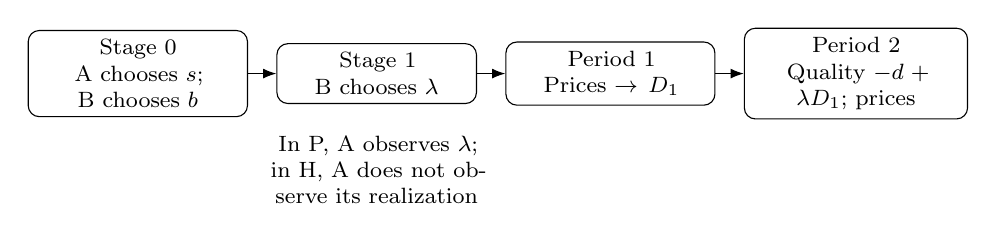
\begin{tikzpicture}[node distance=0.36cm,>=Latex, every node/.style={align=center}]
\node[draw,rounded corners,minimum height=0.75cm,text width=2.55cm,font=\footnotesize] (a) {Stage 0\\A chooses $s$; B chooses $b$};
\node[draw,rounded corners,right=of a,minimum height=0.75cm,text width=2.3cm,font=\footnotesize] (b) {Stage 1\\B chooses $\lambda$};
\node[draw,rounded corners,right=of b,minimum height=0.75cm,text width=2.42cm,font=\footnotesize] (c) {Period 1\\Prices $\to D_1$};
\node[draw,rounded corners,right=of c,minimum height=0.75cm,text width=2.6cm,font=\footnotesize] (d) {Period 2\\Quality $-d+\lambda D_1$; prices};
\draw[->] (a)--(b); \draw[->] (b)--(c); \draw[->] (c)--(d);
\node[below=0.28cm of b,font=\footnotesize,text width=3.6cm] {In P, A observes $\lambda$;\\ in H, A does not observe its realization};
\end{tikzpicture}
\caption{Timing and the information distinction. The incumbent anticipates the hidden equilibrium investment but cannot condition its first-period price on a hidden unilateral deviation.}
\label{fig:timeline}
\end{figure}

We call the two regimes $\PP$ (public) and $\HH$ (hidden). Under $\PP$, A observes the actual choice of $\lambda$ before first-period pricing. Under $\HH$, A's price is measurable with respect to the publicly observed $s,b$ and equilibrium beliefs about $\lambda$, but not B's realized, unobserved investment. B knows its own investment and can reoptimize its first-period price after a deviation. Since second-period quality is publicly observed, the information distinction no longer affects the last price subgame directly. We compare pure-strategy perfect Bayesian equilibria under consistent beliefs, using subgame perfection wherever the continuation is a complete-information proper subgame. Both regimes are otherwise identical.

Let $\pi_{i,k}$ denote firm $i$'s operating profit in period $k$. Net profits are
\begin{equation}
 \Pi_A=\pi_{A,1}+\delta\pi_{A,2}-\frac{k_s}{2}s^2,\qquad
 \Pi_B=\pi_{B,1}+\delta\pi_{B,2}-\frac{k_b}{2}b^2-\frac{\kl}{2}\lambda^2.
 \label{eq:netprofits}
\end{equation}
Social welfare is the discounted sum of consumers' gross quality and transport benefits, less \emph{real} research costs. Prices cancel as transfers. With $D_2$ the entrant's period-2 share and the common base valuation suppressed, this is
\begin{align}
W={}&(1+\delta)s-d(D_1+\delta D_2)+\delta\lambda D_1D_2 \nonumber\\
&-\frac{t}{2}\left[(1-D_1)^2+D_1^2+
 \delta\{(1-D_2)^2+D_2^2\}\right] \nonumber\\
&-\frac{k_s}{2}s^2-\frac{k_b}{2}b^2-\frac{\kl}{2}\lambda^2.
\label{eq:welfare}
\end{align}
We report all equilibrium inequalities with their precise domains; no claim below refers to arbitrary off-equilibrium interior formulas outside their admissible range.

\section{Pricing and the incentive to learn}\label{sec:prices}

We solve the game backward, beginning with the second-period price subgame. Write $q=-d+\lambda D_1$ for B's relative quality. The usual indifferent-consumer equation gives $D_2=[t+q+p_{A,2}-p_{B,2}]/(2t)$.

\begin{lemma}[Dynamic Bertrand prices]\label{lem:prices}
On the full-coverage, strictly interior domain, the period-2 price equilibrium conditional on $q$ is
\begin{equation}
 p_{A,2}^*=t-\frac{q}{3},\quad
 p_{B,2}^*=t+\frac{q}{3},\quad
 D_2^*=\frac{3t+q}{6t}. \label{eq:p2}
\end{equation}
With the firms anticipating the effect of first-period sales on future quality, their period-1 interior price equilibrium, conditional on the relevant information, has entrant market share
\begin{equation}
 D_1^*(d,\lambda)=
 \frac{27t^2-9dt-2\delta d\lambda}
 {2(27t^2-\delta\lambda^2)}, \label{eq:d1}
\end{equation}
and first-period price equations
\begin{align}
p_{A,1}^*&=2t(1-D_1^*)-\frac{\delta\lambda(3t-q)}{9t},\label{eq:p1a}\\
p_{B,1}^*&=2tD_1^*-\frac{\delta\lambda(3t+q)}{9t},\quad q=-d+\lambda D_1^*.\label{eq:p1b}
\end{align}
When $\delta\lambda^2<27t^2$ and all feasibility/interiority conditions hold, these equations select the unique interior price solution.
\end{lemma}

The second-period expressions are standard differentiated Bertrand markups. The first-period prices are not: each firm considers how an extra current sale changes B's future quality. An incumbent that lowers its current price reduces B's current customer base and hence B's next-period competitive strength. The terms proportional to $\delta\lambda$ in \eqref{eq:p1a}--\eqref{eq:p1b} measure this intertemporal incentive. Appendix~\ref{app:prices} gives the first-order conditions and the maintained domain.

Let $V_i(d,\lambda)$ denote the sum of firm $i$'s two operating profits after substituting the price equations, before R\&D costs. A central distinction concerns the derivative of $V_B$ with respect to the entrant's investment when the incumbent is allowed to react to an observed investment versus the payoff to an \emph{unobserved unilateral deviation}.

\begin{proposition}[Observability and learning incentives]\label{prop:incentives}
Suppose $0<d<3t$, $\delta>0$, and evaluate a deviation from $\lambda=0$ on the interior equilibrium branch. Under $\PP$,
\begin{equation}
\left.\frac{\dd V_B^{\PP}}{\dd\lambda}\right|_{\lambda=0}
=-\frac{2\delta d(3t-d)}{81t^2}<0. \label{eq:publicder}
\end{equation}
Under $\HH$, holding A's price strategy fixed under B's unobserved deviation while letting B reoptimize its price,
\begin{equation}
\left.\frac{\partial V_B^{\HH}}{\partial\lambda}\right|_{\lambda=0}
=\frac{\delta(3t-d)^2}{54t^2}>0. \label{eq:hiddender}
\end{equation}
The public-minus-hidden wedge has the strict sign
\begin{equation}
\left.\frac{\partial V_B^{\HH}}{\partial\lambda}
-\frac{\dd V_B^{\PP}}{\dd\lambda}\right|_0
=\frac{\delta(3t-d)(9t+d)}{162t^2}>0. \label{eq:wedge}
\end{equation}
\end{proposition}

The mechanism is a \emph{conditional price threat}. In the public regime,
\begin{equation}
\left.\frac{\partial p_{A,1}^*}{\partial\lambda}\right|_0
=-\frac{\delta(9t+d)}{27t}<0.\label{eq:reaction}
\end{equation}
If the entrant makes its future learning more effective and that action is observed, the incumbent cuts its price, depriving the entrant of the market experience needed to exploit the additional capability. Concealment eliminates this response to an unobserved deviation, although A still correctly anticipates the investment played in equilibrium. Equation~\eqref{eq:reaction} concerns \emph{how A would price if the publicly observed investment changed}; it does not claim that the equilibrium price under P is lower than its level under H. Proof details are in Appendix~\ref{app:prices}.

The marginal signs alone do not establish global investment levels. Nevertheless, they provide an analytically sharp basis for an equilibrium comparison when the cost of learning investment is sufficiently high. Put $\eta=1/\kl$ and define
\begin{equation}
h(d)=\frac{\delta(3t-d)^2}{54t^2}>0. \label{eq:h}
\end{equation}
Under compact, admissible action sets with smoothly varying unique continuation equilibria, the public optimal investment is zero for sufficiently small $\eta$, while the hidden investment is
\begin{equation}
 \lambda^{\HH}(d)=\eta h(d)+O(\eta^2),\qquad
 \lambda^{\PP}(d)=0. \label{eq:lambdahigh}
\end{equation}
The argument compares global payoffs after bounding investments away from zero by the quadratic cost, and then uses the opposite local derivatives in Proposition~\ref{prop:incentives}. Appendix~\ref{app:investment} makes the regularity and scope qualifications explicit.

\section{The direction of R\&D and welfare}\label{sec:results}

We now allow both firms' stage-0 quality choices to adjust. An immediate-quality improvement persists into period 2, but its returns do not depend on the entrant winning customers in period 1. In contrast, the return to $\lambda$ is proportional to the realized customer base. Observability can therefore change the relative attractiveness of these investments.

At $\lambda=0$ define
\begin{equation}
F_A(d)=\frac{(1+\delta)(3t+d)^2}{18t},\quad
F_B(d)=\frac{(1+\delta)(3t-d)^2}{18t},\quad
c=\frac{1+\delta}{9t}. \label{eq:F}
\end{equation}
The stage-0 first-order conditions give $k_s s_*=c(3t+d_*)$ and $k_b b_*=c(3t-d_*)$, where
\begin{equation}
d_*=
\frac{d_0+3tc(k_s^{-1}-k_b^{-1})}
{1-c(k_s^{-1}+k_b^{-1})}. \label{eq:dstar}
\end{equation}
Assume
\begin{equation}
 k_s>c,\quad k_b>c,\quad
 \Delta=k_sk_b-c(k_s+k_b)>0,\quad
 0<d_*<3t, \label{eq:stability}
\end{equation}
and the other interiority/global-continuation regularity conditions stated in Appendix~\ref{app:investment}. These conditions hold at the normalized baseline used below.

\begin{proposition}[A change in the direction of R\&D]\label{prop:composition}
Fix a model with \eqref{eq:stability} and a differentiable, uniquely selected admissible equilibrium continuation around $\eta=0$. For all sufficiently small $\eta>0$,
\begin{equation}
 \lambda^{\HH}>\lambda^{\PP}=0,\qquad
 b^{\HH}<b^{\PP},\qquad
 s^{\HH}>s^{\PP}. \label{eq:composition}
\end{equation}
The strict changes in $s$ and $b$ are of order $\eta$.
\end{proposition}

The intuition is a shift in the \emph{direction} rather than necessarily the total amount of R\&D. Concealment makes learning investment profitable at the margin, so B can rely relatively more on future customer-based improvements and less on improving its quality immediately. A, facing a stronger future entrant, also increases its persistent quality investment in the equilibrium characterized here. Conversely, under disclosure B chooses more immediate quality investment and abandons learning investment in the high-cost region, while A chooses less persistent quality investment. These are independent quadratic research expenditures; no fixed total research budget is assumed. Moreover, A's persistent-quality investment response should not be conflated with its current-price defense.

The general proof is instructive. Set $g_A(d)=\partial_\lambda V_A(d,0)$, $g_B(d)=\partial_\lambda V_B(d,0)$ along the equilibrium price branch and define $u_A=g_Ah$, $u_B=g_Bh-h^2/2$. Expanding stage-0 equilibrium investments as
\begin{equation}
s^{\HH}=s_*+\eta S_1+O(\eta^2),\quad
b^{\HH}=b_*+\eta B_1+O(\eta^2),
\end{equation}
yields
\begin{align}
S_1&=\frac{(k_b-c)u_A'(d_*)+c u_B'(d_*)}{\Delta}>0,\label{eq:scoef}\\
B_1&=-\frac{c u_A'(d_*)+(k_s-c)u_B'(d_*)}{\Delta}<0.\label{eq:bcoef}
\end{align}
Both derivatives $u_A'$ and $u_B'$ are positive for $0<d_*<3t$. Appendix~\ref{app:investment} gives the explicit polynomials and shows the sign. The inequalities in \eqref{eq:composition} therefore do not come from a numerically chosen example, though the scope is a high-learning-cost region.

What happens to profits and welfare is subtler. Greater hidden learning intensifies product-market competition and may reduce firms' profits; consumers may value the accompanying higher future quality and stronger competition. However, the incumbent also benefits under concealment when B cuts its immediate quality investment. It is therefore necessary to specify when that offsetting effect is sufficiently small.

\begin{theorem}[Privately preferred disclosure and socially preferred concealment]\label{thm:main}
Maintain the assumptions of Proposition~\ref{prop:composition} and suppose, in addition, that
\begin{equation}
t\le d_*<3t,\qquad
-B_1<
\frac{\delta(9t-2d_*)}{9t(1+\delta)}\,h(d_*).
\label{eq:Acondition}
\end{equation}
For sufficiently large $\kl$ (equivalently, sufficiently small positive $\eta$), the equilibrium comparisons satisfy
\begin{equation}
 \Pi_A^{\PP}>\Pi_A^{\HH},\qquad
 \Pi_B^{\PP}>\Pi_B^{\HH},\qquad
 W^{\HH}>W^{\PP}. \label{eq:profitwelfare}
\end{equation}
The stated sufficient region is nonempty. The theorem is conditional on an admissible, uniquely selected continuation; no claim is made about arbitrary parameter values or unverified alternative equilibria.
\end{theorem}

The restrictions have economic meaning. When $t\le d_*<3t$, the entrant initially has positive but no more than one-third market share. This makes a larger learning capability particularly relevant to a weaker competitor's attempt to catch up. The second restriction says that the entrant's reduction of immediate quality investment under concealment is not so large that it outweighs the incumbent's disadvantage from facing more learning-based competition. Firm B has an unambiguously negative hidden-profit change to first order; the additional restriction is needed for A. The welfare result follows because the value of enhanced learning and the induced quality changes dominates its real R\&D cost under these sufficient conditions.

To make the accounting transparent, write $CS=W-\Pi_A-\Pi_B$. Equation~\eqref{eq:profitwelfare} implies
\begin{equation}
 CS^{\HH}-CS^{\PP}>
 (\Pi_A^{\PP}-\Pi_A^{\HH})+
 (\Pi_B^{\PP}-\Pi_B^{\HH})>0. \label{eq:cs}
\end{equation}
This is an implication of welfare accounting, not a separate theoretical discovery. Nor does it mean that the firms voluntarily choose the public regime in a disclosure-choice game: the two information environments are fixed exogenously.

\section{Mechanism, finite-cost example, and limits}\label{sec:mechanism}

The general propositions characterize an economic mechanism in a high-learning-cost region. A complementary nonasymptotic calculation establishes that the same sign pattern is not confined to an infinitesimal neighborhood of zero learning.

\subsection{A finite-cost realization}

Normalize $t=\delta=d_0=1$ and $k_s=k_b=4$, and restrict the strategy sets to $s,b\in[0,\frac12]$ and $\lambda\in[0,1]$. The algebraic certificate in the accompanying replication code supports a \emph{sufficient} threshold
\begin{equation}
 \kl>\frac{4343}{32448}\simeq 0.133845 \label{eq:threshold}
\end{equation}
for unique admissible equilibria under each regime with the same investment, profit, and welfare comparisons. The computer-assisted proof uses exact rational Bernstein-coefficient bounds for a cubic equilibrium condition in the quality gap and the relevant payoff signs. Unlike the general high-cost result, this is a \emph{separately specialized finite-domain certificate}, not a simple parameter substitution into Theorem~\ref{thm:main}. A branch-level sign check can be extended to $\kl\ge0.1$, but global equilibrium uniqueness is not established over that entire wider region. The precise scope of the certificate and remaining independent-verification obligations are in Appendix~\ref{app:finite}.

\begin{table}[t]
\centering
\begin{threeparttable}
\caption{Equilibrium outcomes: a finite-cost comparison}
\label{tab:benchmark}
\begin{tabular}{lrr}
\toprule
& Public ($\PP$) & Hidden ($\HH$) \\
\midrule
Incumbent persistent quality $s$ & 0.229167 & 0.252492 \\
Entrant immediate quality $b$ & 0.104167 & 0.096746 \\
Entrant learning capability $\lambda$ & 0 & 0.211102 \\
Entrant share, period 1 ($D_1$) & 0.312500 & 0.298833 \\
Entrant share, period 2 ($D_2$) & 0.312500 & 0.317890 \\
Incumbent net profit $\Pi_A$ & 1.785590 & 1.719007 \\
Entrant net profit $\Pi_B$ & 0.368924 & 0.341936 \\
Welfare $W$ (constant $v$ removed) & $-0.941840$ & $-0.914278$ \\
\bottomrule
\end{tabular}
\begin{tablenotes}[flushleft]\footnotesize
\item Notes: $t=\delta=d_0=1$, $k_s=k_b=4$, $\kl=0.3$. All figures are rounded; payoffs are net of quadratic R\&D expenses. Welfare is measured relative to the same suppressed baseline valuation under both regimes. The associated exact-sign checks are computer-assisted and await independent referee-style audit.
\end{tablenotes}
\end{threeparttable}
\end{table}

The entrant's period-1 share is smaller under concealment, even though its period-2 share is larger. This is a useful empirical interpretation of the model's dynamic incentive: the entrant need not win more current customers for concealed research to improve its future competitiveness. Under the finite-cost certificate, the ranking of the two market shares reverses; the entrant's second-period relative quality and gross market surplus in each period are also higher under H. The claim concerns a two-period comparison, not an indefinite technological replacement process.

The role of endogenous research composition requires a careful qualification. Holding $s$ and $b$ fixed at their public-equilibrium values, and reoptimizing B's hidden learning investment at the same benchmark, gives $\lambda\simeq0.218541$ and welfare $\simeq-0.929585$; permitting all three investments to adjust yields welfare $\simeq-0.914278$, compared with public welfare $\simeq-0.941840$. Thus the welfare reversal occurs \emph{even with quality R\&D fixed}, while the endogenous adjustment of quality R\&D amplifies it in this example. The fixed-$(s,b)$ calculation is a counterfactual, \emph{not} a full-game equilibrium. No general amplification theorem is claimed.

\subsection{Why experience feedback matters}

To isolate the economic channel, consider replacing the learning technology in \eqref{eq:technology} by
\begin{equation}
q_{B,2}=b-d_0+\lambda. \label{eq:nofeedback}
\end{equation}
In this controlled alternative, second-period quality no longer depends on first-period sales. First-period prices therefore cannot affect the value of future learning. With publicly observed period-2 realized quality and otherwise identical assumptions, first-period prices coincide across observability institutions; the Stage-1 investment objective and, under uniqueness, the Stage-0 equilibrium also coincide. The public-hidden wedge disappears. This is a conditional mechanism-removal argument rather than a claim about all possible disclosure or learning models. Its complete formalization remains an audit task.

The two principal margins should also be distinguished. A's price reaction to \emph{more observed learning} is negative [equation~\eqref{eq:reaction}], but the \emph{public-equilibrium} incumbent price can be higher than the hidden-equilibrium price because the equilibrium investments differ. For the benchmark, $p_{A,1}^{\PP}=1.375$ while $p_{A,1}^{\HH}\simeq1.30634$. Confusing the derivative with a cross-regime comparison would lead to an incorrect interpretation.

Several restrictions delimit the result. First, information observability is exogenously assigned, not voluntarily selected. Second, research expenses have independent quadratic costs; they are not financed from a common fixed laboratory budget. Third, consumers are myopic and locations fixed. Fourth, the finite-cost threshold is specific to the stated normalization and compact strategy sets. These are deliberate boundaries of the present analysis, not hidden robustness claims.

\section{Conclusion}\label{sec:conclusion}

Information about a firm's future learning capability can change the value of that capability precisely because market experience is determined competitively. In a two-period differentiated Bertrand game, the incumbent's conditional current-price defense can discourage an entrant from investing in the ability to learn. Allowing the firms to adjust immediate and persistent quality R\&D then redirects the innovation mix. Under explicit sufficient conditions, disclosure raises both firms' equilibrium profits even though concealment yields higher social welfare and, in the finite-cost example, a stronger future entrant.

The broader lesson is not that R\&D disclosure is universally undesirable. It is that a disclosure institution can shape the direction of technological change through product-market strategic responses, even in the absence of patents, information spillovers or capital-market short-termism. The exact boundary of this result outside the stated admissible and certified domains, and its independence from all related general theorems, remain subjects of the ongoing mathematical and literature audits.

\appendix
\section{Price subgames and the observability wedge}\label{app:prices}

The entrant's first-period demand is
\begin{equation}
D_1=\frac{t-d+p_{A,1}-p_{B,1}}{2t}. \label{eq:demanda}
\end{equation}
For a relative period-2 quality $q$, the static pricing first-order conditions give \eqref{eq:p2} and
\[
\pi_{A,2}=\frac{(3t-q)^2}{18t},\qquad
\pi_{B,2}=\frac{(3t+q)^2}{18t}.
\]
Let $q=-d+\lambda D_1$, and substitute the second-period optimized profits into the period-1 objectives. Differentiation of $p_{A,1}(1-D_1)+\delta\pi_{A,2}(q)$ and $p_{B,1}D_1+\delta\pi_{B,2}(q)$ yields the price equations in Lemma~\ref{lem:prices}. Simultaneous solution gives \eqref{eq:d1}. Each firm's own-price objective is strictly concave for $\delta\lambda^2<27t^2$, conditional on the maintained interior domain; the linear FOC system is nonsingular there. Additional demand/price inequalities must be checked before using the interior solution globally.

Substitute the price equilibria into gross continuation profits:
\begin{align*}
V_A(d,\lambda)&=p_{A,1}^*(1-D_1^*)+
 \delta\frac{(3t-q)^2}{18t},\\
V_B(d,\lambda)&=p_{B,1}^*D_1^*+
 \delta\frac{(3t+q)^2}{18t}.
\end{align*}
The total derivative along the public price-equilibrium path gives equation~\eqref{eq:publicder}. For hidden $\lambda$, hold A's price at the price chosen under its equilibrium belief, while reoptimizing B's price conditional on B's true $\lambda$. At $\lambda=0$, the envelope theorem gives the right derivative \eqref{eq:hiddender}. The difference \eqref{eq:wedge} is algebraic. These derivatives are evaluated at zero investment and do not claim that each public/hidden equilibrium payoff function is globally ordered for all $\lambda$.

\section{High-cost equilibrium expansion}\label{app:investment}

Write $\eta=\kl^{-1}$ and fix a compact action domain on which all relevant price continuations are feasible, unique, smooth, and their gross payoffs bounded. For $\eta$ sufficiently close to zero, the quadratic $\lambda^2/(2\eta)$ makes positive investment bounded away from zero strictly unprofitable. At $\lambda=0$, the public right derivative of B's gross payoff is negative by Proposition~\ref{prop:incentives}, and the hidden derivative is positive. Thus for high cost the public optimum is zero and the hidden hidden-deviation optimality condition yields
\[
\lambda^{\HH}=\eta h(d)+O(\eta^2),\qquad
h(d)=\frac{\delta(3t-d)^2}{54t^2}.
\]
The statement about global optimality requires the above boundedness, uniform local derivative and second-order conditions, rather than only a first-order condition at zero.

Define
\begin{align}
g_A(d)&=-\frac{\delta(9t-2d)(3t+d)}{81t^2},\nonumber\\
g_B(d)&=-\frac{2\delta d(3t-d)}{81t^2},\qquad
u_A=g_Ah,\quad u_B=g_Bh-\tfrac12h^2.
\label{eq:ug}
\end{align}
After substituting the hidden Stage-1 policy, the two gross continuation values with B's learning cost deducted in the second are
\[
T_A^{\HH}(d)=F_A(d)+\eta u_A(d)+O(\eta^2),
\quad
T_B^{\HH}(d)=F_B(d)+\eta u_B(d)+O(\eta^2).
\]
The derivatives needed to sign the stage-0 adjustment are
\begin{align}
u_A'(d)&=
\frac{\delta^2(3t-d)(-8d^2+21dt+45t^2)}
{4374t^4}>0,\label{eq:upa}\\
u_B'(d)&=
\frac{\delta^2(3t-d)^2(5d+3t)}
{4374t^4}>0,\qquad 0<d<3t.\label{eq:upb}
\end{align}
At zero learning the Stage-0 FOCs are $k_s s_*=F_A'(d_*)$ and $k_b b_*=-F_B'(d_*)$; since $F_A''=F_B''=c$, their Jacobian is
\[
J=\begin{pmatrix}k_s-c&c\\c&k_b-c\end{pmatrix},
\qquad \det J=\Delta>0.
\]
Applying the implicit-function theorem at the no-learning equilibrium,
\[
J\begin{pmatrix}S_1\\B_1\end{pmatrix}=
\begin{pmatrix}u_A'(d_*)\\-u_B'(d_*)\end{pmatrix},
\]
gives equations~\eqref{eq:scoef}--\eqref{eq:bcoef}. The derivatives are strictly signed by \eqref{eq:upa}--\eqref{eq:upb}. This construction is a regular equilibrium-branch argument; global full-game uniqueness requires the separate continuation and deviation controls maintained in the propositions.

\section{Profit and welfare sign decomposition}\label{app:welfare}

The leading hidden-minus-public \emph{net} profit coefficients are
\begin{align}
\Pi_A^{\HH}-\Pi_A^{\PP}
 &=\eta\underbrace{\left[u_A(d_*)-F_A'(d_*)B_1\right]}_{\Phi_A}
  +O(\eta^2),\label{eq:pacoef}\\
\Pi_B^{\HH}-\Pi_B^{\PP}
 &=\eta\underbrace{\left[u_B(d_*)+F_B'(d_*)S_1\right]}_{\Phi_B}
  +O(\eta^2).\label{eq:pbcoef}
\end{align}
Here $u_B<0$, $F_B'<0$, and $S_1>0$ for $0<d_*<3t$, so $\Phi_B<0$ without another restriction. For A, $\Phi_A<0$ exactly when condition~\eqref{eq:Acondition} holds. This condition prevents the competitive benefit to A from B's reduced immediate quality under concealment from overcoming A's loss from stronger future learning competition.

Differentiating \eqref{eq:welfare} at $\lambda=0$ along the price equilibrium gives
\[
W_\lambda(d,0)=
\frac{\delta(23d^2-72dt+81t^2)}{324t^2}.
\]
At the baseline R\&D equilibrium, the derivatives of welfare with respect to the investments are
\[
W_s=\frac{(1+\delta)(t+d_*)}{6t},\qquad
W_b=\frac{(1+\delta)(t-d_*)}{6t}.
\]
Including the first-order learning cost, the leading welfare difference is
\begin{align}
W^{\HH}-W^{\PP}
=\eta\Bigg\{&
h(d_*)\frac{\delta(10d_*^2-27d_*t+27t^2)}{162t^2}\nonumber\\
&+\frac{1+\delta}{6t}
\left[(t+d_*)S_1+(t-d_*)B_1\right]
\Bigg\}+O(\eta^2).\label{eq:wcoef}
\end{align}
The quadratic $10d_*^2-27d_*t+27t^2$ has a negative discriminant and positive leading coefficient, hence is strictly positive. For $t\le d_*<3t$, the $S_1$ term is positive and the $B_1$ term nonnegative. Thus the bracket is strictly positive. Since the leading profit coefficients are strictly negative under the theorem's additional condition, the inequalities survive sufficiently small positive $\eta$.

To see that the stated parameter region need not be a single isolated point, consider $t=\delta=d_0=1$ and $k_s=k_b=K$ for $K\ge4$. Then $d_*=9K/(9K-4)$ lies in $(1,9/8]$, and direct rational-algebra evaluation of the incumbent-profit restriction gives the required strict sign; its strictness persists in an open neighborhood. The supporting polynomial calculations are documented in the research record and must receive independent proof auditing before a submission-level theorem claim.

\section{Exact symbolic finite-cost certificate and scope}\label{app:finite}

Set $t=\delta=d_0=1$, $k_s=k_b=4$, and impose the compact strategy sets indicated in Section~\ref{sec:mechanism}. Writing $D=D_1$, the equilibrium branch is described by
\[
D=\frac{27-(9+2\lambda)d}{2(27-\lambda^2)},\qquad
q=-d+\lambda D,
\]
and hidden Stage-1 optimality yields the rational function
\begin{equation}
\kl=K(d,\lambda):=
\frac{
[27-(9+2\lambda)d]\,
[54-18d+(9-3d)\lambda-2\lambda^2]
}
{12\lambda(27-\lambda^2)^2}.
\label{eq:K}
\end{equation}
Let $V_A,V_B$ be the operating profits from Lemma~\ref{lem:prices} under the normalized parameters and define
\[
\mathcal D f=\partial_d f-\frac{K_d}{K_\lambda}\partial_\lambda f.
\]
Then the induced quality investments satisfy
\[
 s=\tfrac14\mathcal D V_A,\quad
 b=-\tfrac14\mathcal D(V_B-\kl\lambda^2/2),\quad
 d=1+s-b.
\]
After clearing denominators, the last equation reduces to a cubic polynomial in $d$ with coefficients polynomial in $\lambda$. The exact verification program, \texttt{code/finite\_cost\_proof.py}, checks the related cubic-root wedge
\[
\frac98+\frac{\lambda}{8}<d(\lambda)<
\frac98+\frac{\lambda}{5},
\qquad 0<\lambda\le\tfrac12,
\]
and the relevant R\&D/profit/welfare signs using rational Bernstein coefficients on a unit square. It also verifies derivative bounds underlying the sufficient global-equilibrium threshold~\eqref{eq:threshold} in the stated compact domain. The program separately checks a larger \emph{equilibrium-branch} sign region corresponding to $\kl\ge0.1$, without establishing global equilibrium uniqueness on the entire expanded domain.

\textbf{Certification disclosure.} These computations have been reproduced, but the exhaustive off-path continuation audit, independent clean-room equilibrium reconstruction, and proof-assistant applicability/closure required by the project's workflow remain outstanding. Until then, finite-cost uniqueness and sign claims are \emph{computer-assisted research results}, not independently certified submission claims. The script and its stdout log, plus the source repository, preserve the reproducibility trail. Neither numerical root finding alone nor positivity on a selected branch would justify an unrestricted SPNE assertion.

\section{A feedback-removal diagnostic}\label{app:ablation}
If the alternative technology \eqref{eq:nofeedback} replaces \eqref{eq:technology}, first-period prices no longer enter any future operating payoff. The first-period price subgame is static and independent of $\lambda$, while the second-period price equilibrium depends only on the realized second-period quality difference. At Stage 1 the entrant's objective, conditional on $d$, is thus the same function of $\lambda$ in both information regimes. When these continuation objectives and the earlier R\&D equilibrium are uniquely optimized, public and hidden choices coincide. This argument concerns removal of \emph{market-share feedback}; it does not rule out disclosure effects in other games with private technical types, signaling, commitment or direct dynamic cost effects.

\bibliographystyle{plainnat}
\bibliography{references}
\end{document}
